% Options for packages loaded elsewhere
\PassOptionsToPackage{unicode}{hyperref}
\PassOptionsToPackage{hyphens}{url}
%
\documentclass[
]{article}
\usepackage{amsmath,amssymb}
\usepackage{iftex}
\ifPDFTeX
  \usepackage[T1]{fontenc}
  \usepackage[utf8]{inputenc}
  \usepackage{textcomp} % provide euro and other symbols
\else % if luatex or xetex
  \usepackage{unicode-math} % this also loads fontspec
  \defaultfontfeatures{Scale=MatchLowercase}
  \defaultfontfeatures[\rmfamily]{Ligatures=TeX,Scale=1}
\fi
\usepackage{lmodern}
\ifPDFTeX\else
  % xetex/luatex font selection
\fi
% Use upquote if available, for straight quotes in verbatim environments
\IfFileExists{upquote.sty}{\usepackage{upquote}}{}
\IfFileExists{microtype.sty}{% use microtype if available
  \usepackage[]{microtype}
  \UseMicrotypeSet[protrusion]{basicmath} % disable protrusion for tt fonts
}{}
\makeatletter
\@ifundefined{KOMAClassName}{% if non-KOMA class
  \IfFileExists{parskip.sty}{%
    \usepackage{parskip}
  }{% else
    \setlength{\parindent}{0pt}
    \setlength{\parskip}{6pt plus 2pt minus 1pt}}
}{% if KOMA class
  \KOMAoptions{parskip=half}}
\makeatother
\usepackage{xcolor}
\usepackage[margin=1in]{geometry}
\usepackage{color}
\usepackage{fancyvrb}
\newcommand{\VerbBar}{|}
\newcommand{\VERB}{\Verb[commandchars=\\\{\}]}
\DefineVerbatimEnvironment{Highlighting}{Verbatim}{commandchars=\\\{\}}
% Add ',fontsize=\small' for more characters per line
\usepackage{framed}
\definecolor{shadecolor}{RGB}{248,248,248}
\newenvironment{Shaded}{\begin{snugshade}}{\end{snugshade}}
\newcommand{\AlertTok}[1]{\textcolor[rgb]{0.94,0.16,0.16}{#1}}
\newcommand{\AnnotationTok}[1]{\textcolor[rgb]{0.56,0.35,0.01}{\textbf{\textit{#1}}}}
\newcommand{\AttributeTok}[1]{\textcolor[rgb]{0.13,0.29,0.53}{#1}}
\newcommand{\BaseNTok}[1]{\textcolor[rgb]{0.00,0.00,0.81}{#1}}
\newcommand{\BuiltInTok}[1]{#1}
\newcommand{\CharTok}[1]{\textcolor[rgb]{0.31,0.60,0.02}{#1}}
\newcommand{\CommentTok}[1]{\textcolor[rgb]{0.56,0.35,0.01}{\textit{#1}}}
\newcommand{\CommentVarTok}[1]{\textcolor[rgb]{0.56,0.35,0.01}{\textbf{\textit{#1}}}}
\newcommand{\ConstantTok}[1]{\textcolor[rgb]{0.56,0.35,0.01}{#1}}
\newcommand{\ControlFlowTok}[1]{\textcolor[rgb]{0.13,0.29,0.53}{\textbf{#1}}}
\newcommand{\DataTypeTok}[1]{\textcolor[rgb]{0.13,0.29,0.53}{#1}}
\newcommand{\DecValTok}[1]{\textcolor[rgb]{0.00,0.00,0.81}{#1}}
\newcommand{\DocumentationTok}[1]{\textcolor[rgb]{0.56,0.35,0.01}{\textbf{\textit{#1}}}}
\newcommand{\ErrorTok}[1]{\textcolor[rgb]{0.64,0.00,0.00}{\textbf{#1}}}
\newcommand{\ExtensionTok}[1]{#1}
\newcommand{\FloatTok}[1]{\textcolor[rgb]{0.00,0.00,0.81}{#1}}
\newcommand{\FunctionTok}[1]{\textcolor[rgb]{0.13,0.29,0.53}{\textbf{#1}}}
\newcommand{\ImportTok}[1]{#1}
\newcommand{\InformationTok}[1]{\textcolor[rgb]{0.56,0.35,0.01}{\textbf{\textit{#1}}}}
\newcommand{\KeywordTok}[1]{\textcolor[rgb]{0.13,0.29,0.53}{\textbf{#1}}}
\newcommand{\NormalTok}[1]{#1}
\newcommand{\OperatorTok}[1]{\textcolor[rgb]{0.81,0.36,0.00}{\textbf{#1}}}
\newcommand{\OtherTok}[1]{\textcolor[rgb]{0.56,0.35,0.01}{#1}}
\newcommand{\PreprocessorTok}[1]{\textcolor[rgb]{0.56,0.35,0.01}{\textit{#1}}}
\newcommand{\RegionMarkerTok}[1]{#1}
\newcommand{\SpecialCharTok}[1]{\textcolor[rgb]{0.81,0.36,0.00}{\textbf{#1}}}
\newcommand{\SpecialStringTok}[1]{\textcolor[rgb]{0.31,0.60,0.02}{#1}}
\newcommand{\StringTok}[1]{\textcolor[rgb]{0.31,0.60,0.02}{#1}}
\newcommand{\VariableTok}[1]{\textcolor[rgb]{0.00,0.00,0.00}{#1}}
\newcommand{\VerbatimStringTok}[1]{\textcolor[rgb]{0.31,0.60,0.02}{#1}}
\newcommand{\WarningTok}[1]{\textcolor[rgb]{0.56,0.35,0.01}{\textbf{\textit{#1}}}}
\usepackage{graphicx}
\makeatletter
\def\maxwidth{\ifdim\Gin@nat@width>\linewidth\linewidth\else\Gin@nat@width\fi}
\def\maxheight{\ifdim\Gin@nat@height>\textheight\textheight\else\Gin@nat@height\fi}
\makeatother
% Scale images if necessary, so that they will not overflow the page
% margins by default, and it is still possible to overwrite the defaults
% using explicit options in \includegraphics[width, height, ...]{}
\setkeys{Gin}{width=\maxwidth,height=\maxheight,keepaspectratio}
% Set default figure placement to htbp
\makeatletter
\def\fps@figure{htbp}
\makeatother
\setlength{\emergencystretch}{3em} % prevent overfull lines
\providecommand{\tightlist}{%
  \setlength{\itemsep}{0pt}\setlength{\parskip}{0pt}}
\setcounter{secnumdepth}{-\maxdimen} % remove section numbering
\ifLuaTeX
  \usepackage{selnolig}  % disable illegal ligatures
\fi
\IfFileExists{bookmark.sty}{\usepackage{bookmark}}{\usepackage{hyperref}}
\IfFileExists{xurl.sty}{\usepackage{xurl}}{} % add URL line breaks if available
\urlstyle{same}
\hypersetup{
  pdftitle={BINF-F401},
  hidelinks,
  pdfcreator={LaTeX via pandoc}}

\title{BINF-F401}
\author{}
\date{\vspace{-2.5em}2024-04-08}

\begin{document}
\maketitle

\begin{verbatim}
## -- Attaching core tidyverse packages ------------------------ tidyverse 2.0.0 --
## v dplyr     1.1.2     v readr     2.1.4
## v forcats   1.0.0     v stringr   1.5.0
## v ggplot2   3.4.3     v tibble    3.2.1
## v lubridate 1.9.2     v tidyr     1.3.0
## v purrr     1.0.2     
## -- Conflicts ------------------------------------------ tidyverse_conflicts() --
## x dplyr::filter() masks stats::filter()
## x dplyr::lag()    masks stats::lag()
## i Use the conflicted package (<http://conflicted.r-lib.org/>) to force all conflicts to become errors
## corrplot 0.92 loaded
## 
## 
## Attachement du package : 'gridExtra'
## 
## 
## L'objet suivant est masqué depuis 'package:dplyr':
## 
##     combine
\end{verbatim}

\begin{verbatim}
## Warning: le package 'caret' a été compilé avec la version R 4.3.3
\end{verbatim}

\begin{verbatim}
## Le chargement a nécessité le package : lattice
## 
## Attachement du package : 'caret'
## 
## L'objet suivant est masqué depuis 'package:purrr':
## 
##     lift
\end{verbatim}

\begin{verbatim}
## Warning: le package 'FactoMineR' a été compilé avec la version R 4.3.3
\end{verbatim}

\begin{verbatim}
## Warning: le package 'factoextra' a été compilé avec la version R 4.3.3
\end{verbatim}

\begin{verbatim}
## Welcome! Want to learn more? See two factoextra-related books at https://goo.gl/ve3WBa
\end{verbatim}

\hypertarget{binf-f401-project-r-markdown}{%
\section{BINF-F401 project (R
Markdown)}\label{binf-f401-project-r-markdown}}

The task assigned was to study the RNA expression of a set of patients.

First, let's set the parameters used throughout the scripts.

\begin{Shaded}
\begin{Highlighting}[]
\NormalTok{  p\_value }\OtherTok{=}\NormalTok{ .}\DecValTok{05}
\end{Highlighting}
\end{Shaded}

\hypertarget{description-of-the-clinical_scale-dataframe}{%
\subsection{Description of the clinical\_scale
dataframe}\label{description-of-the-clinical_scale-dataframe}}

The clinical scale dataframe gather the information surrounding the
patients included in the study. Some variables are related to the
patient's physical condition (Age, Sex, Height and Weight), some are
related to its death condition (On ventilator or not, type of death) and
finally some are related to the cell tissue removal (ischemic time,
origin of the cell: organ donor or death in hospital).

\begin{verbatim}
## Rows: 465 Columns: 14
## -- Column specification --------------------------------------------------------
## Delimiter: "\t"
## chr (6): SMPLID, SUBJID, COHORT, SMPTHNTS, SMPLID.1, IMGURL
## dbl (8): SEX, AGE, HGHT, WGHT, BMI, TRISCHD, DTHVNT, DTHHRDY
## 
## i Use `spec()` to retrieve the full column specification for this data.
## i Specify the column types or set `show_col_types = FALSE` to quiet this message.
\end{verbatim}

\hypertarget{distribution-of-the-numerical-variables}{%
\subsubsection{Distribution of the numerical
variables}\label{distribution-of-the-numerical-variables}}

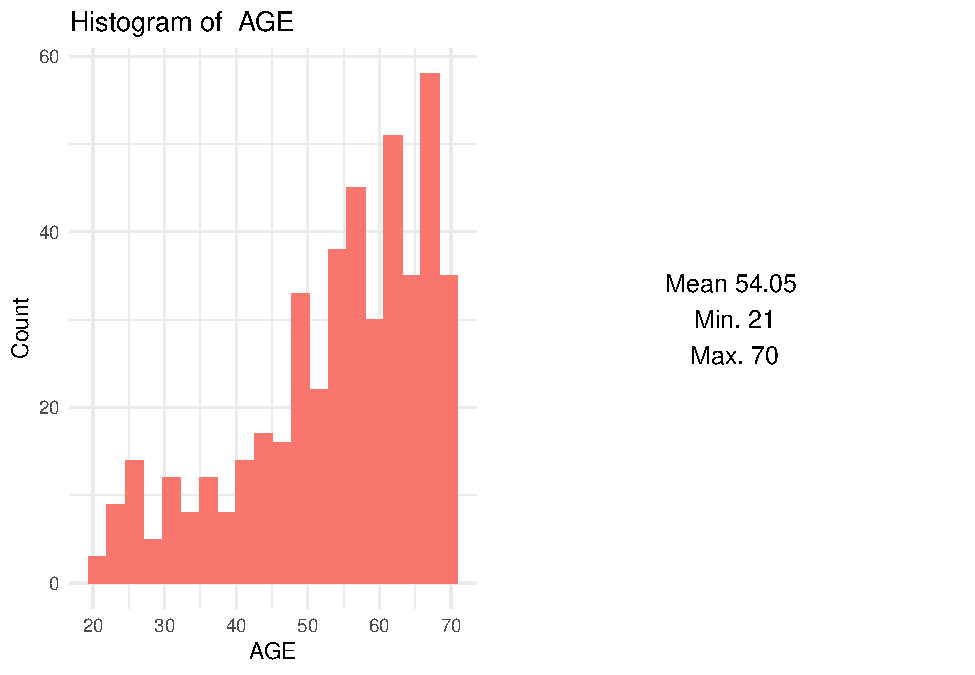
\includegraphics{Q1_markdown_files/figure-latex/unnamed-chunk-4-1.pdf}
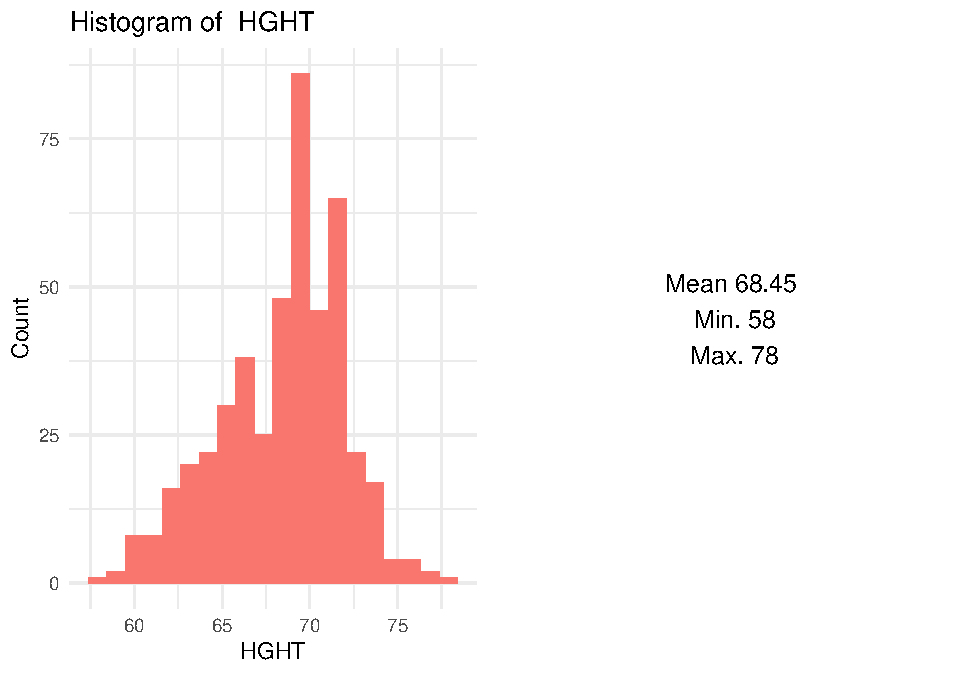
\includegraphics{Q1_markdown_files/figure-latex/unnamed-chunk-4-2.pdf}
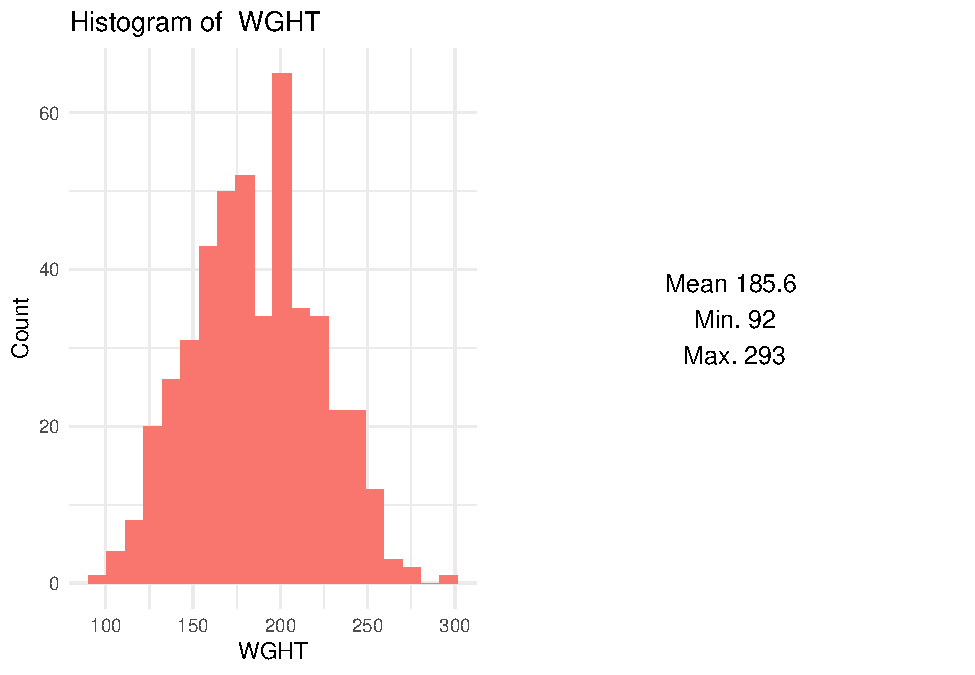
\includegraphics{Q1_markdown_files/figure-latex/unnamed-chunk-4-3.pdf}
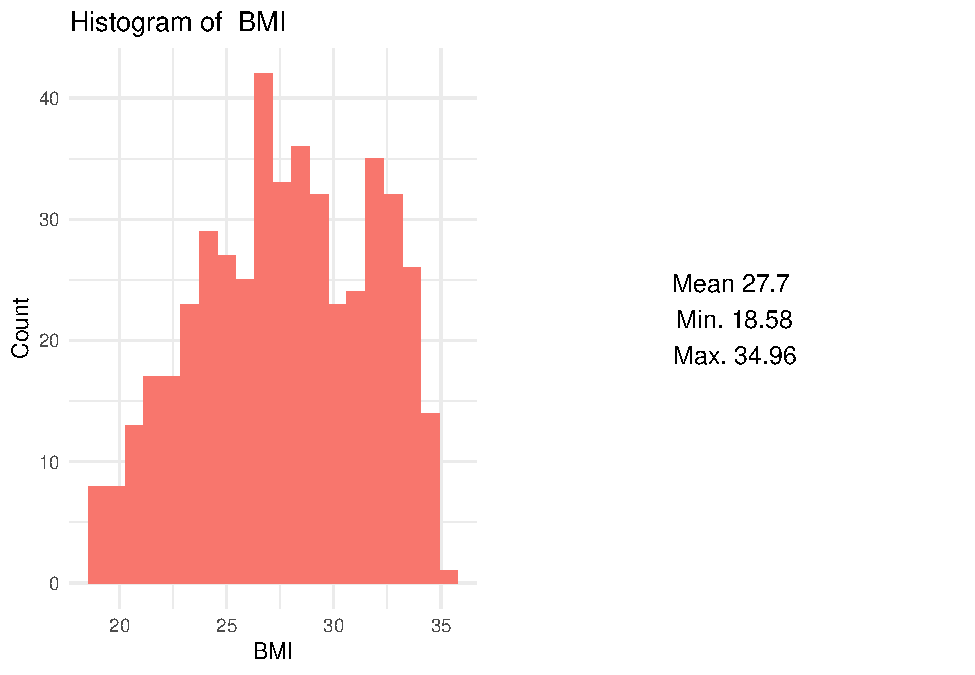
\includegraphics{Q1_markdown_files/figure-latex/unnamed-chunk-4-4.pdf}
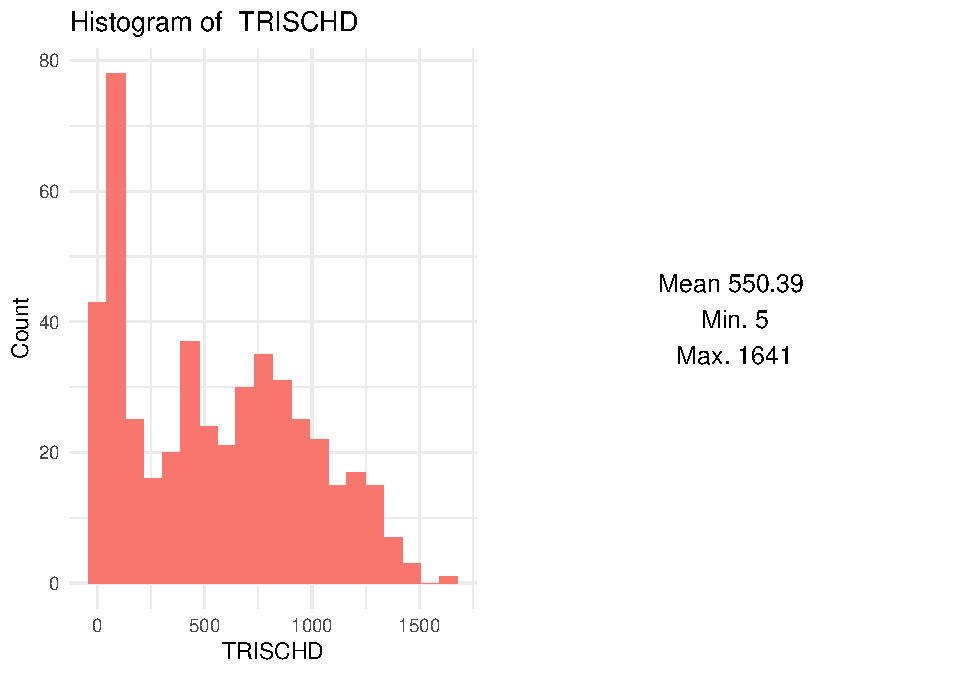
\includegraphics{Q1_markdown_files/figure-latex/unnamed-chunk-4-5.pdf}

\hypertarget{distribution-of-the-binary-variables}{%
\subsubsection{Distribution of the binary
variables}\label{distribution-of-the-binary-variables}}

\begin{verbatim}
## Warning: Use of `clin_bin[[var]]` is discouraged.
## i Use `.data[[var]]` instead.
## Use of `clin_bin[[var]]` is discouraged.
## i Use `.data[[var]]` instead.
\end{verbatim}

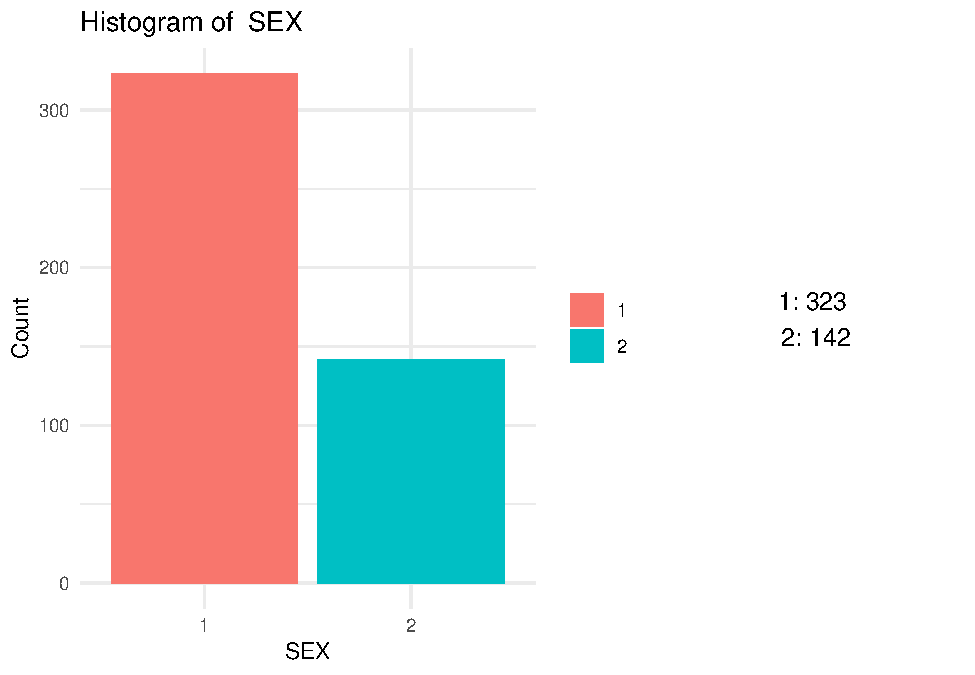
\includegraphics{Q1_markdown_files/figure-latex/unnamed-chunk-5-1.pdf}

\begin{verbatim}
## Warning: Use of `clin_bin[[var]]` is discouraged.
## i Use `.data[[var]]` instead.
## Use of `clin_bin[[var]]` is discouraged.
## i Use `.data[[var]]` instead.
\end{verbatim}

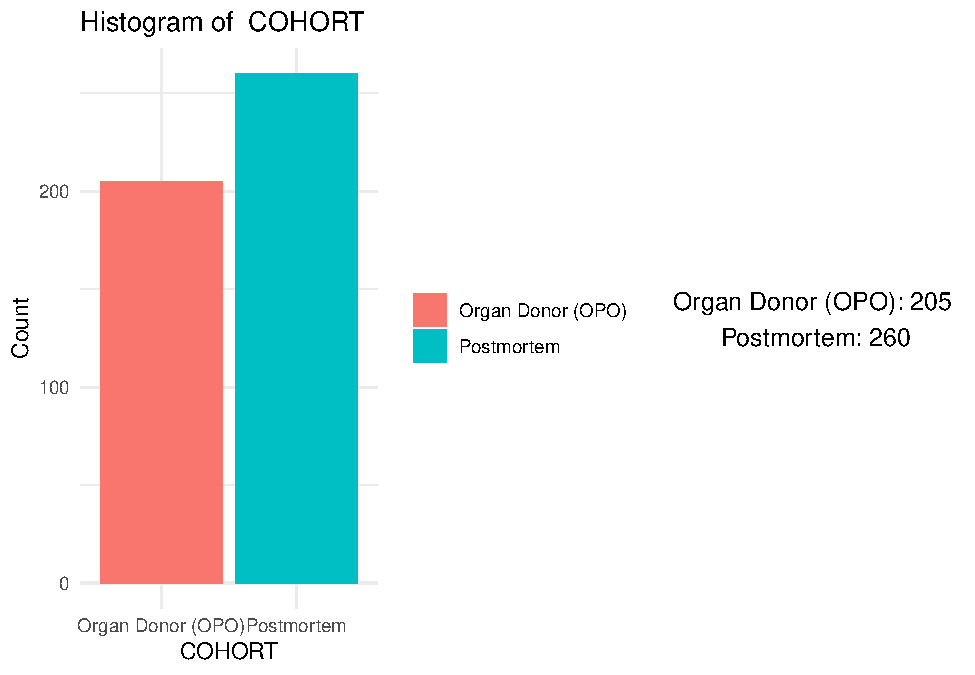
\includegraphics{Q1_markdown_files/figure-latex/unnamed-chunk-5-2.pdf}

\begin{verbatim}
## Warning: Use of `clin_bin[[var]]` is discouraged.
## i Use `.data[[var]]` instead.
## Use of `clin_bin[[var]]` is discouraged.
## i Use `.data[[var]]` instead.
\end{verbatim}

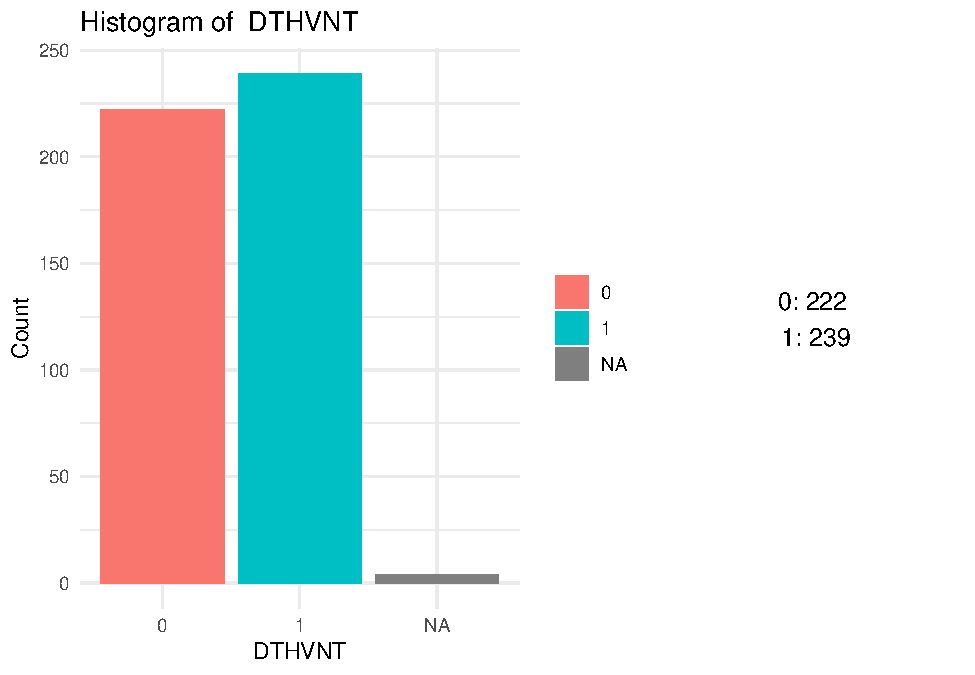
\includegraphics{Q1_markdown_files/figure-latex/unnamed-chunk-5-3.pdf}

\begin{verbatim}
## Warning: Use of `clin_bin[[var]]` is discouraged.
## i Use `.data[[var]]` instead.
## Use of `clin_bin[[var]]` is discouraged.
## i Use `.data[[var]]` instead.
\end{verbatim}

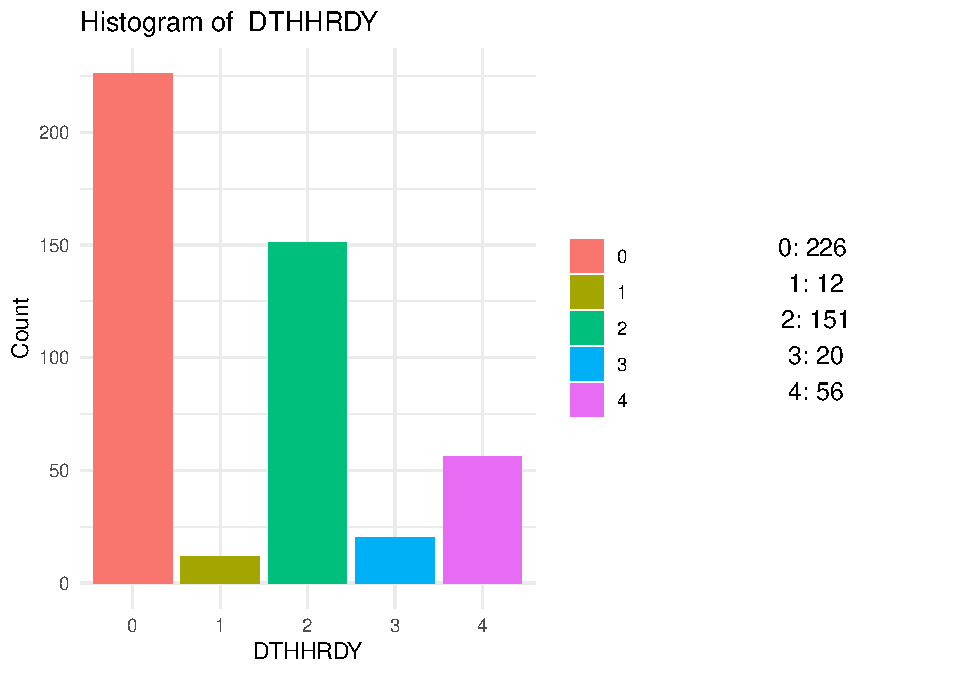
\includegraphics{Q1_markdown_files/figure-latex/unnamed-chunk-5-4.pdf}

\hypertarget{correlations-between-numerical-variables}{%
\subsubsection{Correlations between numerical
variables}\label{correlations-between-numerical-variables}}

\begin{verbatim}
## Warning: Using an external vector in selections was deprecated in tidyselect 1.1.0.
## i Please use `all_of()` or `any_of()` instead.
##   # Was:
##   data %>% select(clinical_numeric)
## 
##   # Now:
##   data %>% select(all_of(clinical_numeric))
## 
## See <https://tidyselect.r-lib.org/reference/faq-external-vector.html>.
## This warning is displayed once every 8 hours.
## Call `lifecycle::last_lifecycle_warnings()` to see where this warning was
## generated.
\end{verbatim}

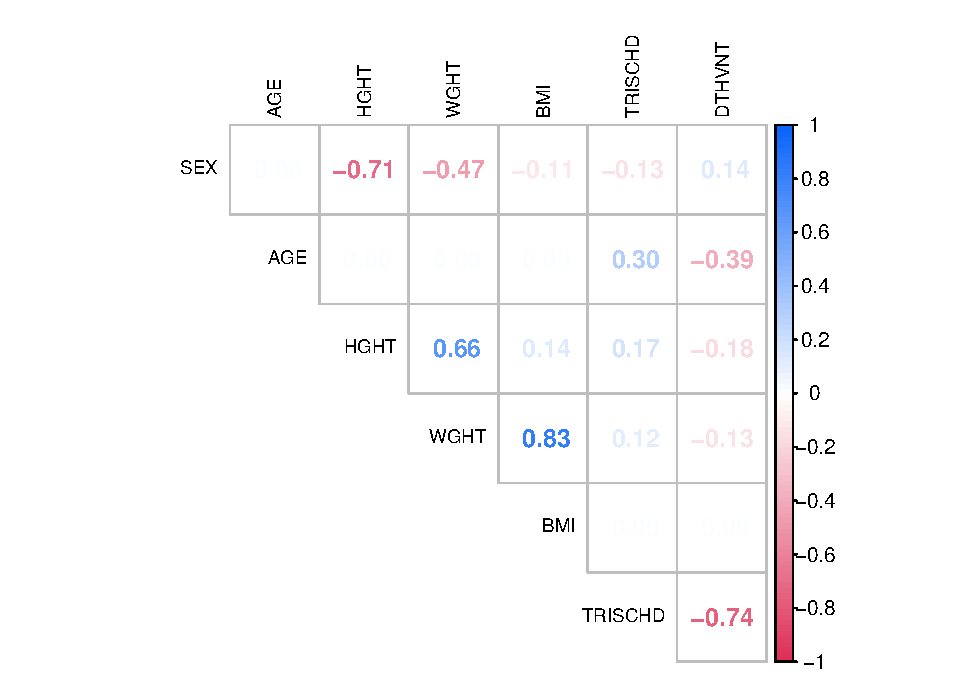
\includegraphics{Q1_markdown_files/figure-latex/unnamed-chunk-6-1.pdf}

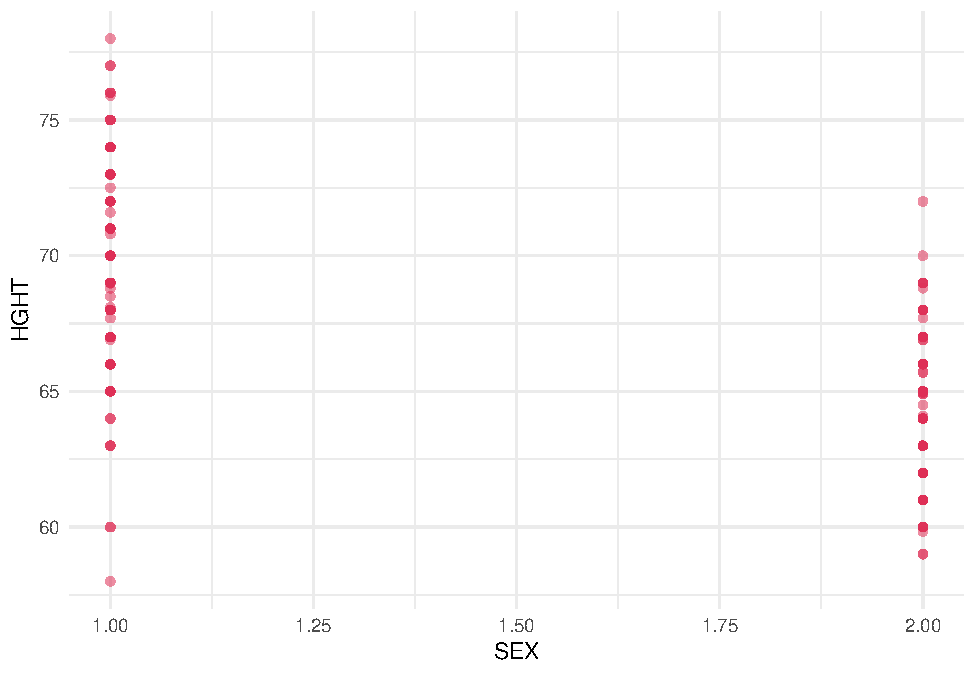
\includegraphics{Q1_markdown_files/figure-latex/unnamed-chunk-7-1.pdf}
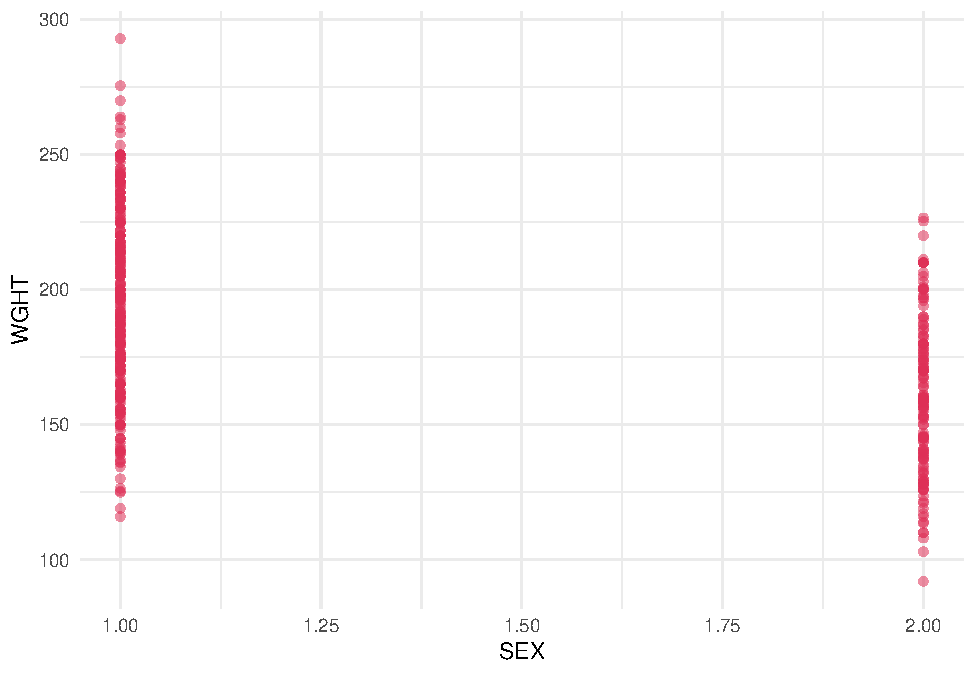
\includegraphics{Q1_markdown_files/figure-latex/unnamed-chunk-7-2.pdf}
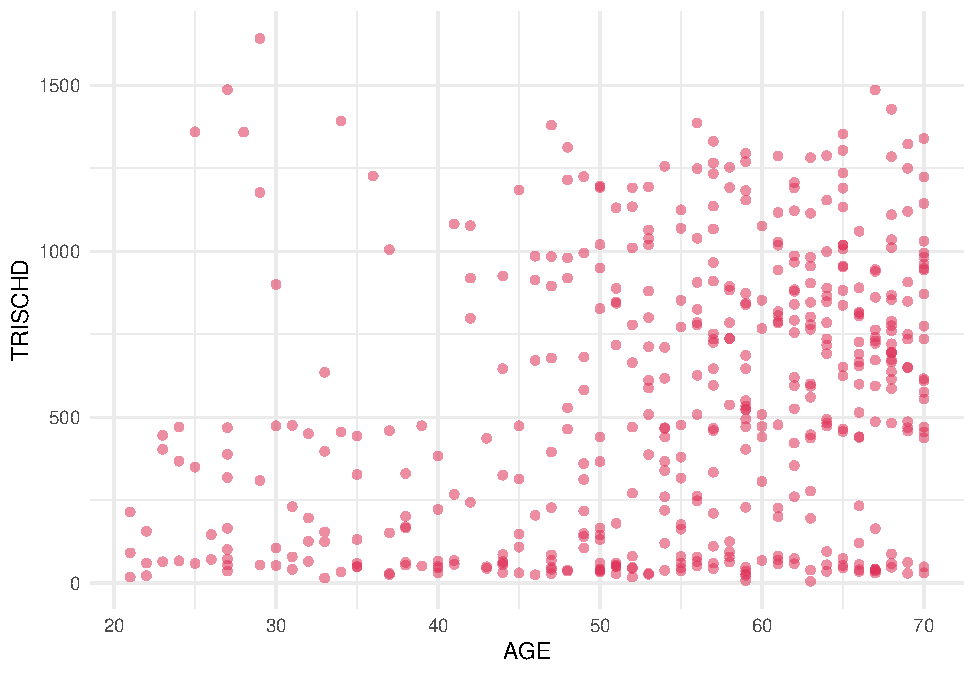
\includegraphics{Q1_markdown_files/figure-latex/unnamed-chunk-7-3.pdf}

\begin{verbatim}
## Warning: Removed 4 rows containing missing values (`geom_point()`).
\end{verbatim}

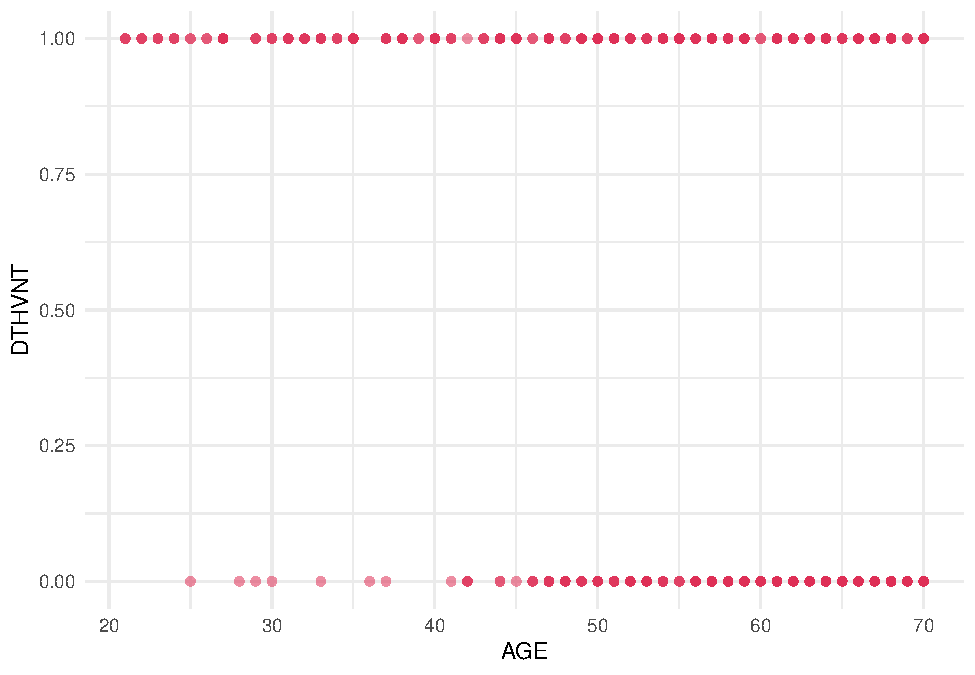
\includegraphics{Q1_markdown_files/figure-latex/unnamed-chunk-7-4.pdf}
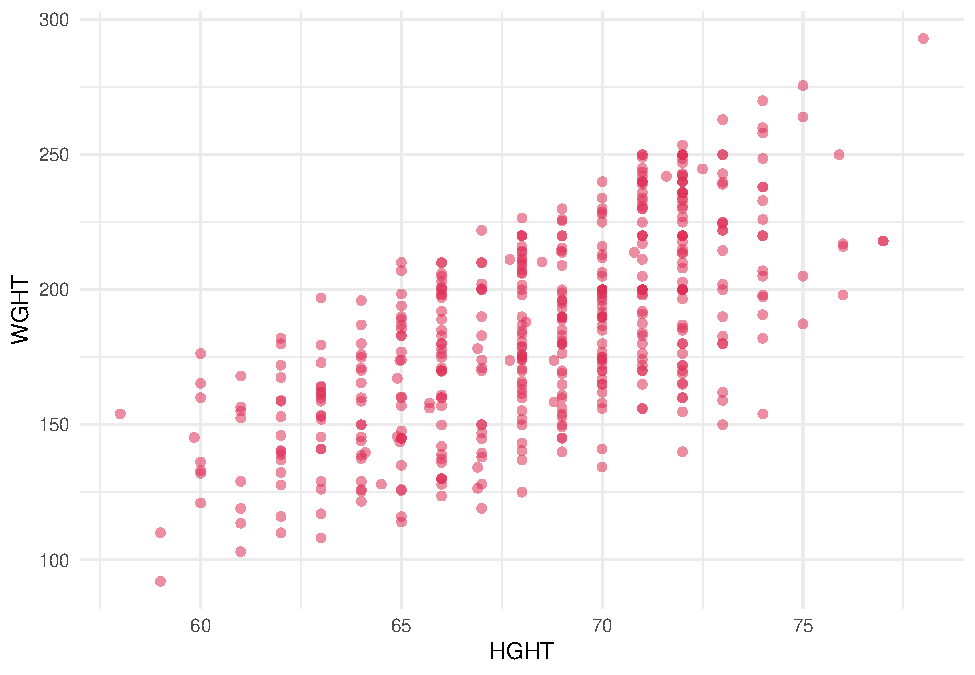
\includegraphics{Q1_markdown_files/figure-latex/unnamed-chunk-7-5.pdf}
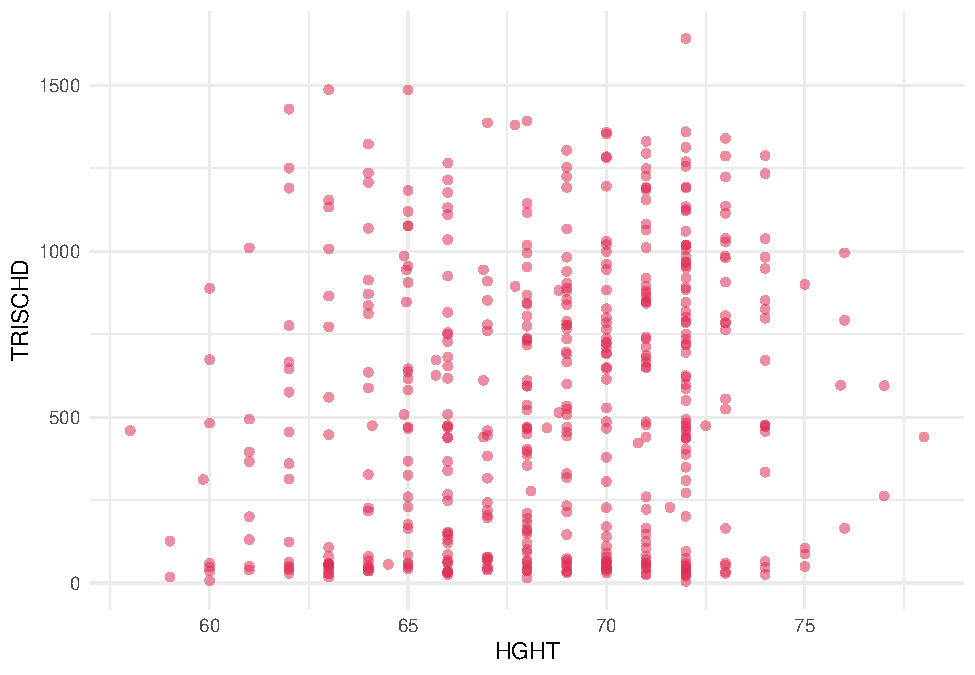
\includegraphics{Q1_markdown_files/figure-latex/unnamed-chunk-7-6.pdf}

\begin{verbatim}
## Warning: Removed 4 rows containing missing values (`geom_point()`).
\end{verbatim}

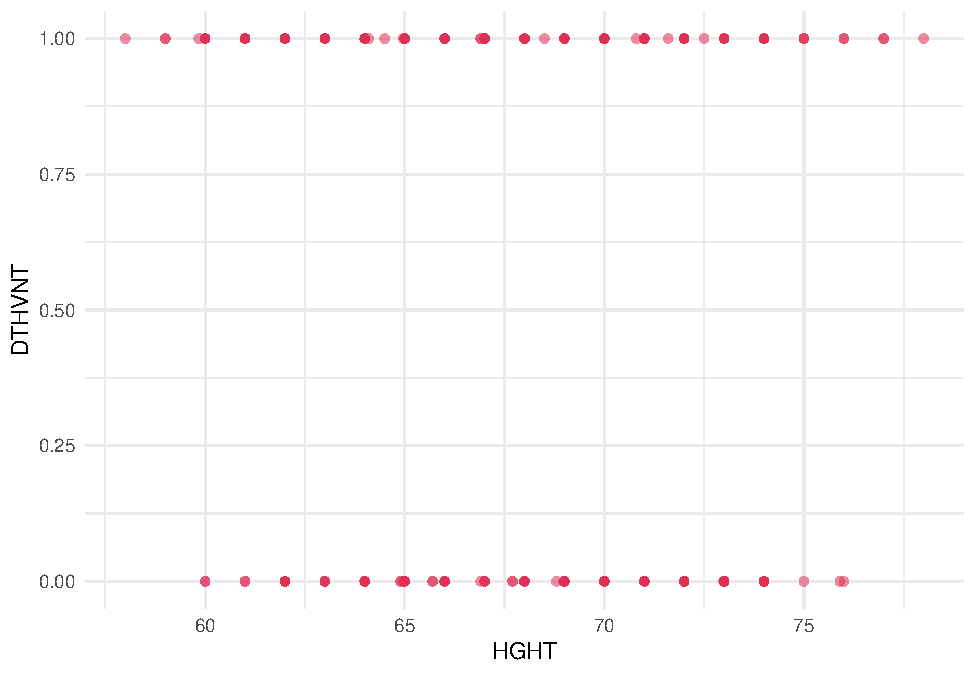
\includegraphics{Q1_markdown_files/figure-latex/unnamed-chunk-7-7.pdf}
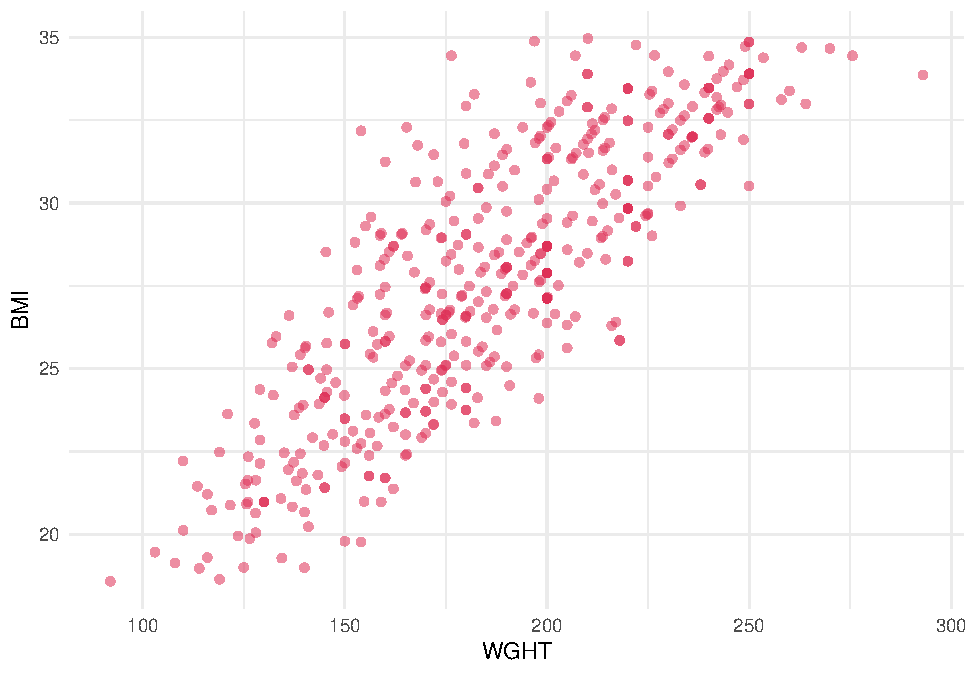
\includegraphics{Q1_markdown_files/figure-latex/unnamed-chunk-7-8.pdf}

\begin{verbatim}
## Warning: Removed 4 rows containing missing values (`geom_point()`).
\end{verbatim}

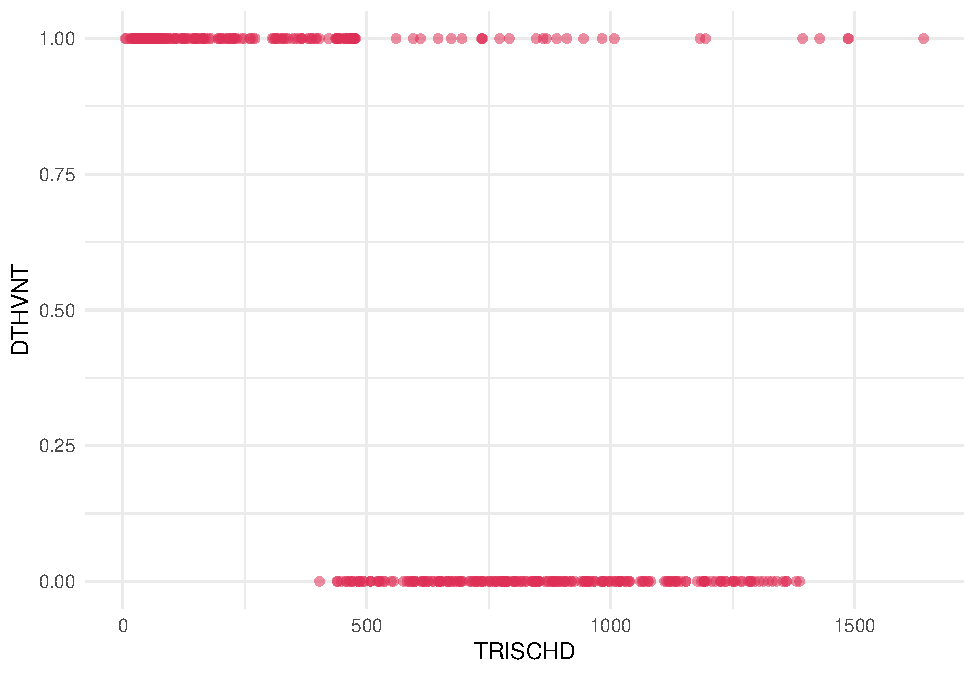
\includegraphics{Q1_markdown_files/figure-latex/unnamed-chunk-7-9.pdf}

\hypertarget{boxplots-of-categorical-variables-against-numerical}{%
\subsubsection{Boxplots of categorical variables against
numerical}\label{boxplots-of-categorical-variables-against-numerical}}

\begin{verbatim}
## Warning: Using an external vector in selections was deprecated in tidyselect 1.1.0.
## i Please use `all_of()` or `any_of()` instead.
##   # Was:
##   data %>% select(var.x)
## 
##   # Now:
##   data %>% select(all_of(var.x))
## 
## See <https://tidyselect.r-lib.org/reference/faq-external-vector.html>.
## This warning is displayed once every 8 hours.
## Call `lifecycle::last_lifecycle_warnings()` to see where this warning was
## generated.
\end{verbatim}

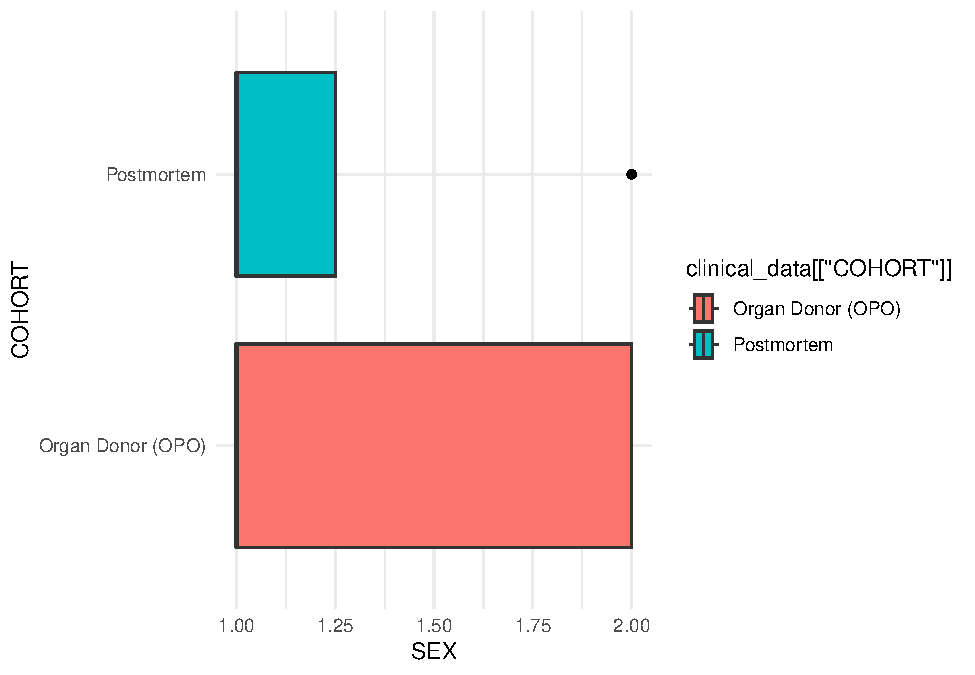
\includegraphics{Q1_markdown_files/figure-latex/unnamed-chunk-8-1.pdf}
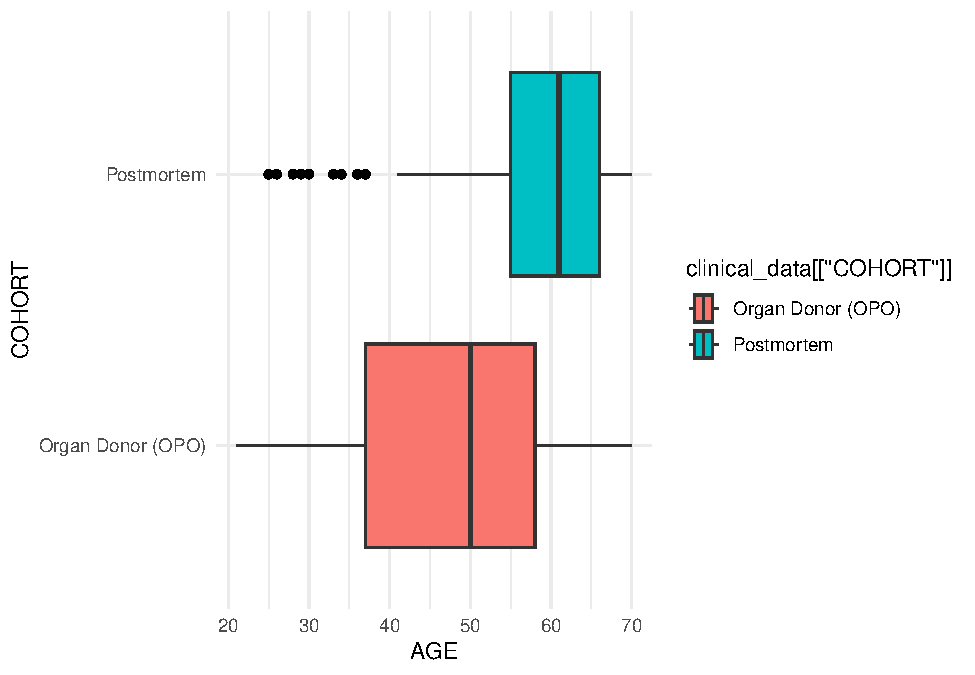
\includegraphics{Q1_markdown_files/figure-latex/unnamed-chunk-8-2.pdf}
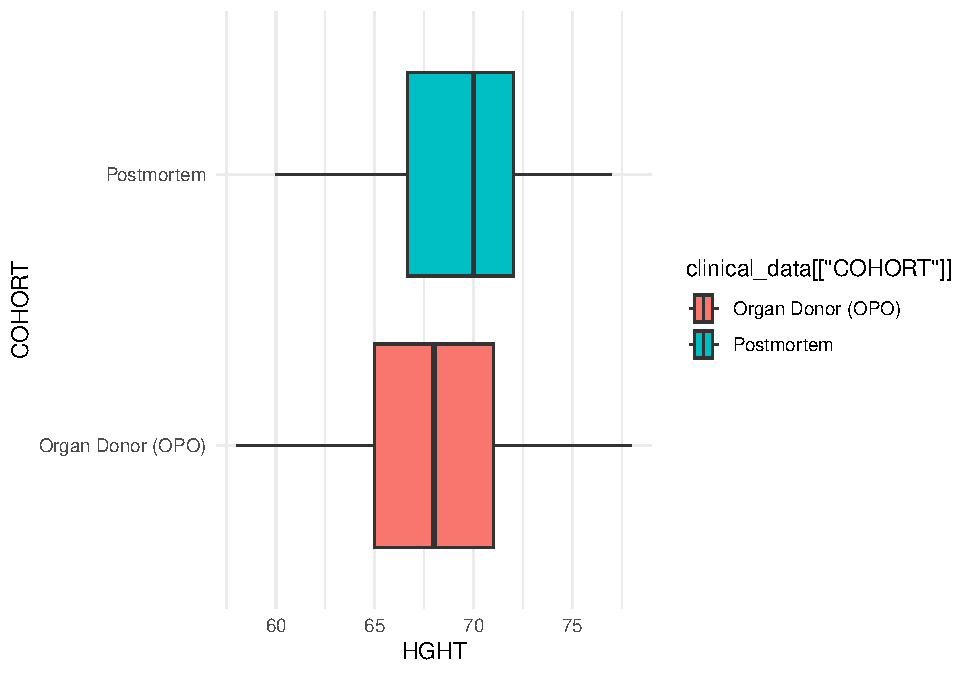
\includegraphics{Q1_markdown_files/figure-latex/unnamed-chunk-8-3.pdf}
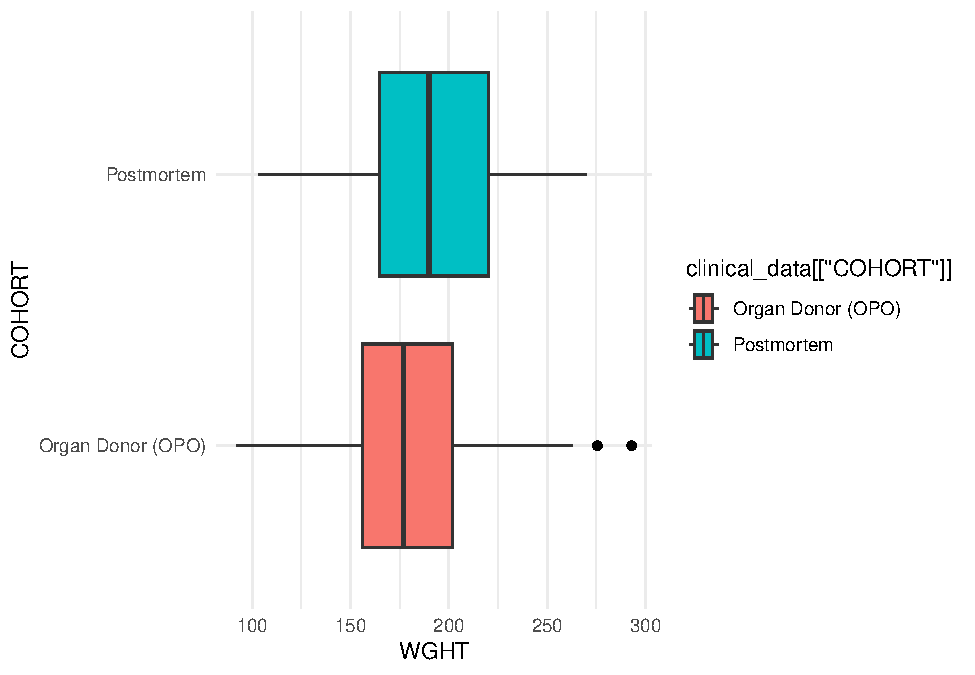
\includegraphics{Q1_markdown_files/figure-latex/unnamed-chunk-8-4.pdf}
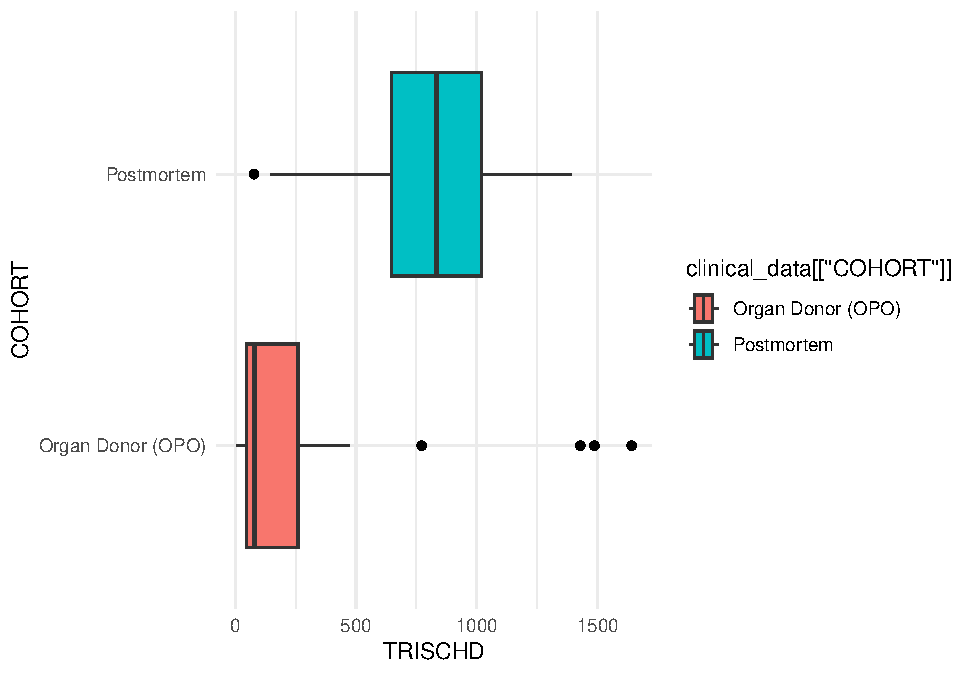
\includegraphics{Q1_markdown_files/figure-latex/unnamed-chunk-8-5.pdf}

\begin{verbatim}
## Warning: Removed 4 rows containing non-finite values (`stat_boxplot()`).
\end{verbatim}

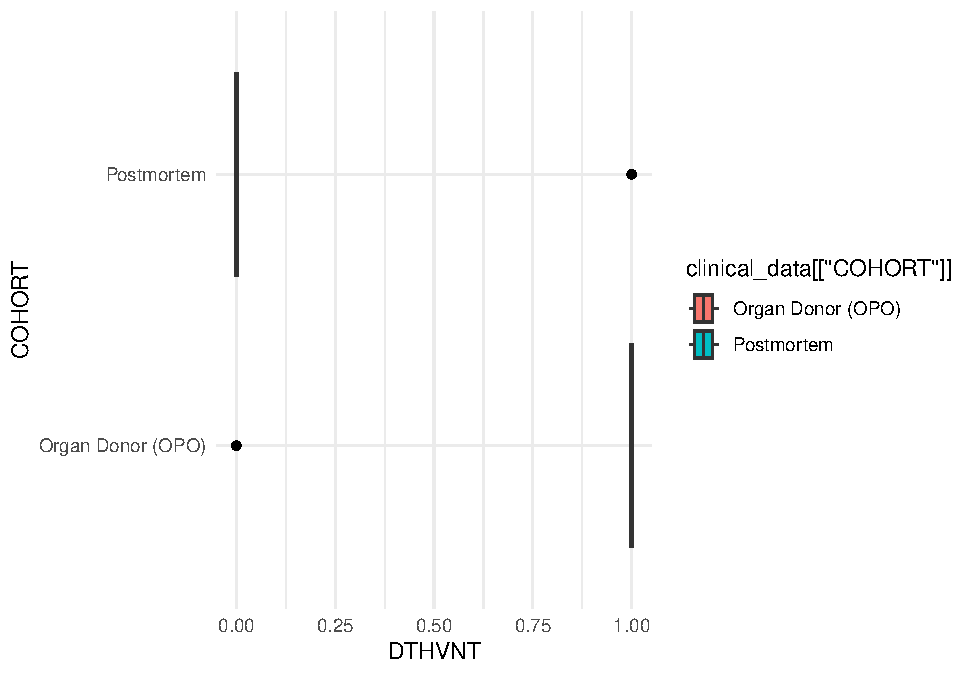
\includegraphics{Q1_markdown_files/figure-latex/unnamed-chunk-8-6.pdf}

\begin{verbatim}
## Warning in model.response(mf, "numeric"): l'utilisation de type="numeric" avec
## une réponse de type facteur sera ignorée
\end{verbatim}

\begin{verbatim}
## Warning in Ops.factor(y, z$residuals): '-' n'est pas pertinent pour des
## variables facteurs
\end{verbatim}

\begin{verbatim}
## Warning in model.response(mf, "numeric"): l'utilisation de type="numeric" avec
## une réponse de type facteur sera ignorée
\end{verbatim}

\begin{verbatim}
## Warning in Ops.factor(y, z$residuals): '-' n'est pas pertinent pour des
## variables facteurs
\end{verbatim}

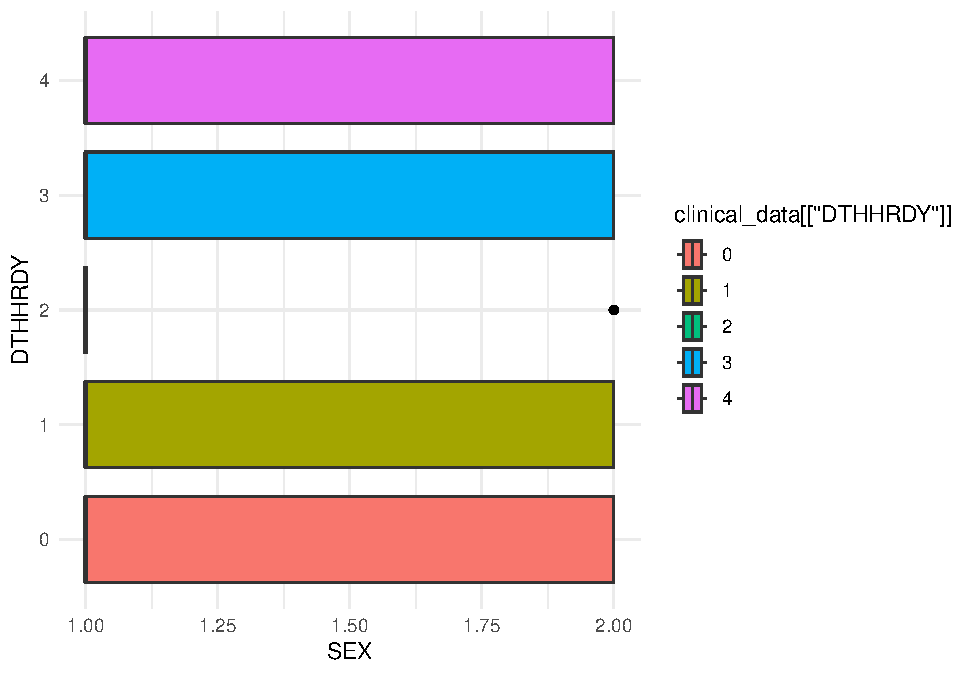
\includegraphics{Q1_markdown_files/figure-latex/unnamed-chunk-8-7.pdf}

\begin{verbatim}
## Warning in model.response(mf, "numeric"): l'utilisation de type="numeric" avec
## une réponse de type facteur sera ignorée

## Warning in model.response(mf, "numeric"): '-' n'est pas pertinent pour des
## variables facteurs
\end{verbatim}

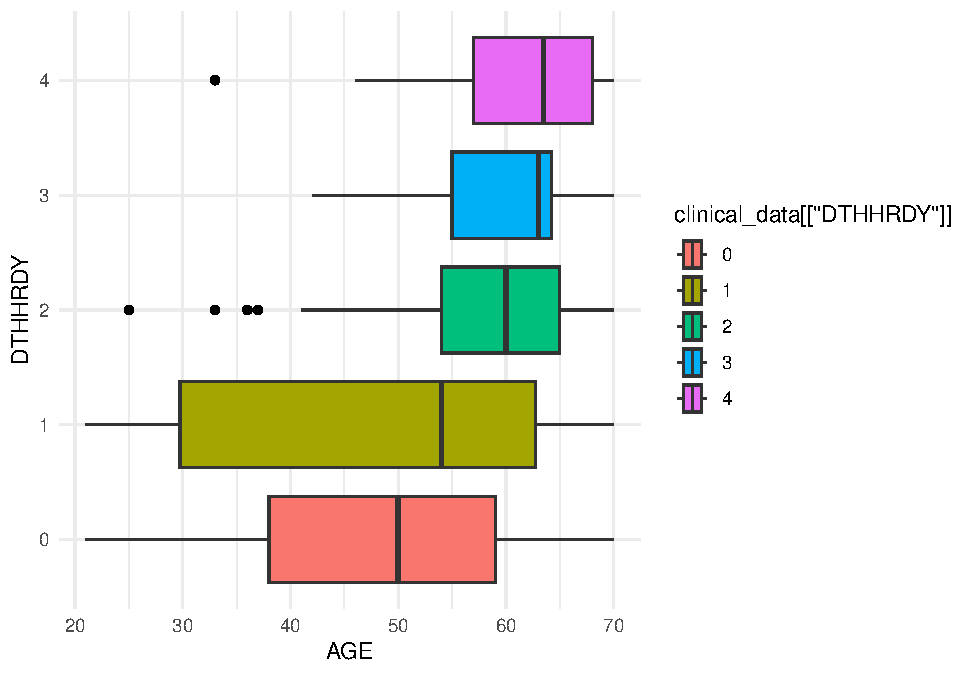
\includegraphics{Q1_markdown_files/figure-latex/unnamed-chunk-8-8.pdf}

\begin{verbatim}
## Warning in model.response(mf, "numeric"): l'utilisation de type="numeric" avec
## une réponse de type facteur sera ignorée

## Warning in model.response(mf, "numeric"): '-' n'est pas pertinent pour des
## variables facteurs
\end{verbatim}

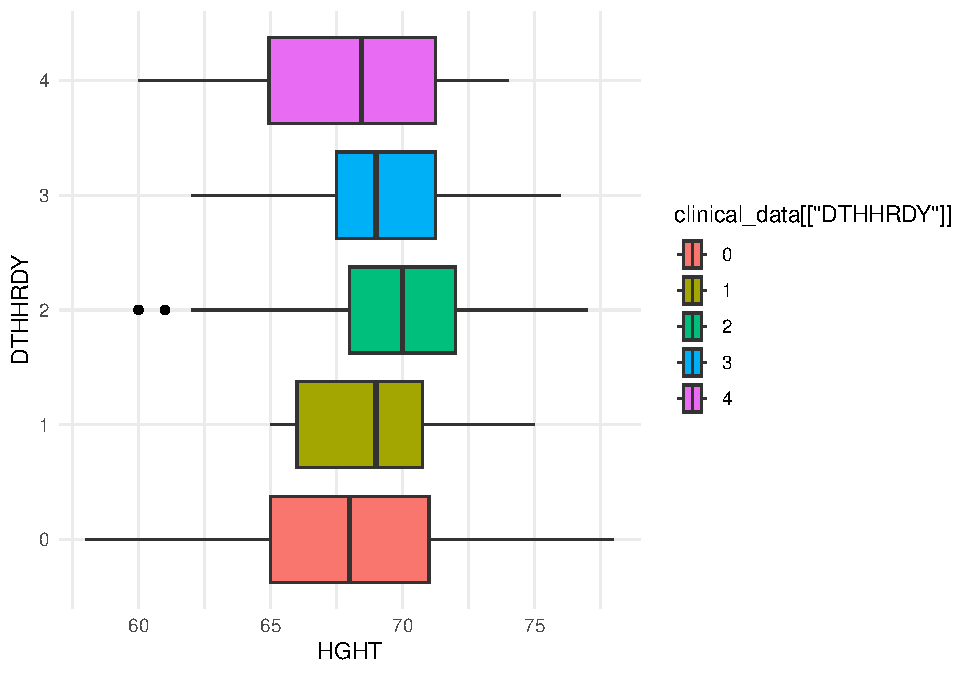
\includegraphics{Q1_markdown_files/figure-latex/unnamed-chunk-8-9.pdf}

\begin{verbatim}
## Warning in model.response(mf, "numeric"): l'utilisation de type="numeric" avec
## une réponse de type facteur sera ignorée

## Warning in model.response(mf, "numeric"): '-' n'est pas pertinent pour des
## variables facteurs
\end{verbatim}

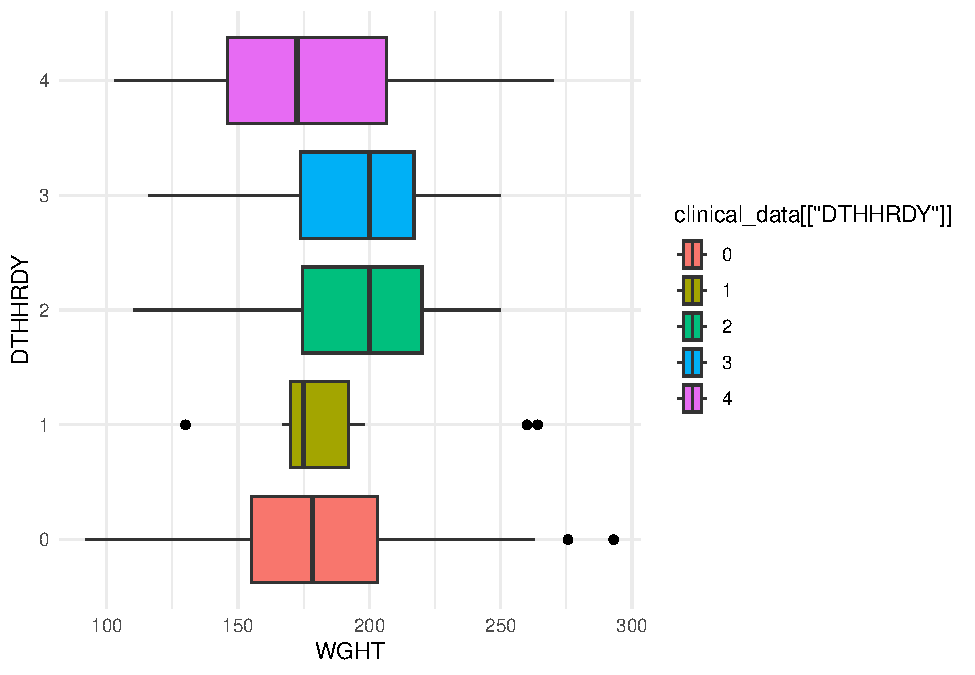
\includegraphics{Q1_markdown_files/figure-latex/unnamed-chunk-8-10.pdf}

\begin{verbatim}
## Warning in model.response(mf, "numeric"): l'utilisation de type="numeric" avec
## une réponse de type facteur sera ignorée

## Warning in model.response(mf, "numeric"): '-' n'est pas pertinent pour des
## variables facteurs
\end{verbatim}

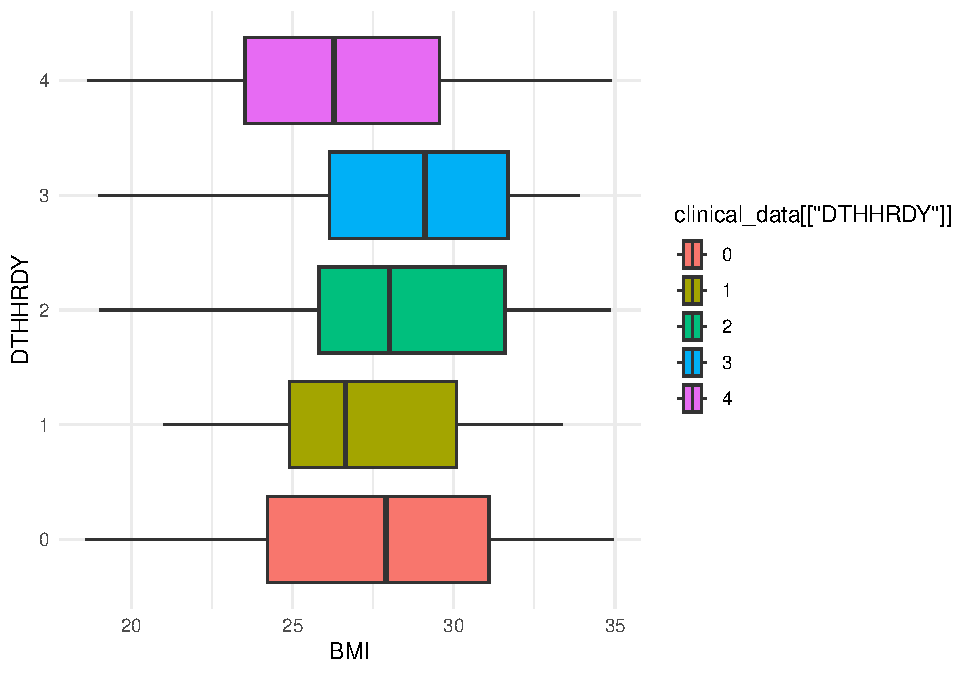
\includegraphics{Q1_markdown_files/figure-latex/unnamed-chunk-8-11.pdf}

\begin{verbatim}
## Warning in model.response(mf, "numeric"): l'utilisation de type="numeric" avec
## une réponse de type facteur sera ignorée

## Warning in model.response(mf, "numeric"): '-' n'est pas pertinent pour des
## variables facteurs
\end{verbatim}

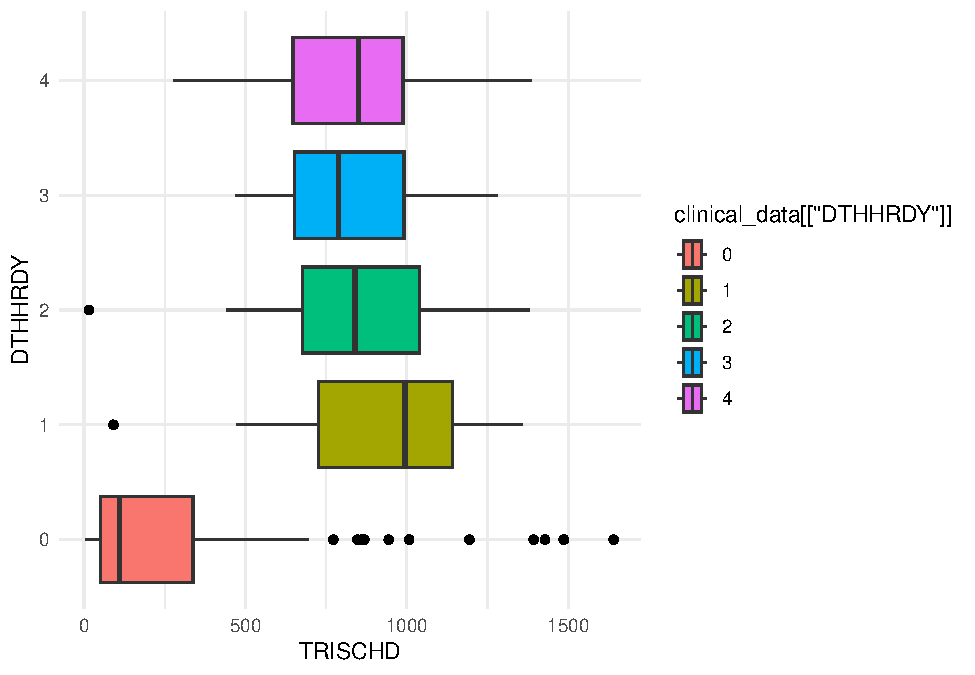
\includegraphics{Q1_markdown_files/figure-latex/unnamed-chunk-8-12.pdf}

\begin{verbatim}
## Warning: Removed 4 rows containing non-finite values (`stat_boxplot()`).
\end{verbatim}

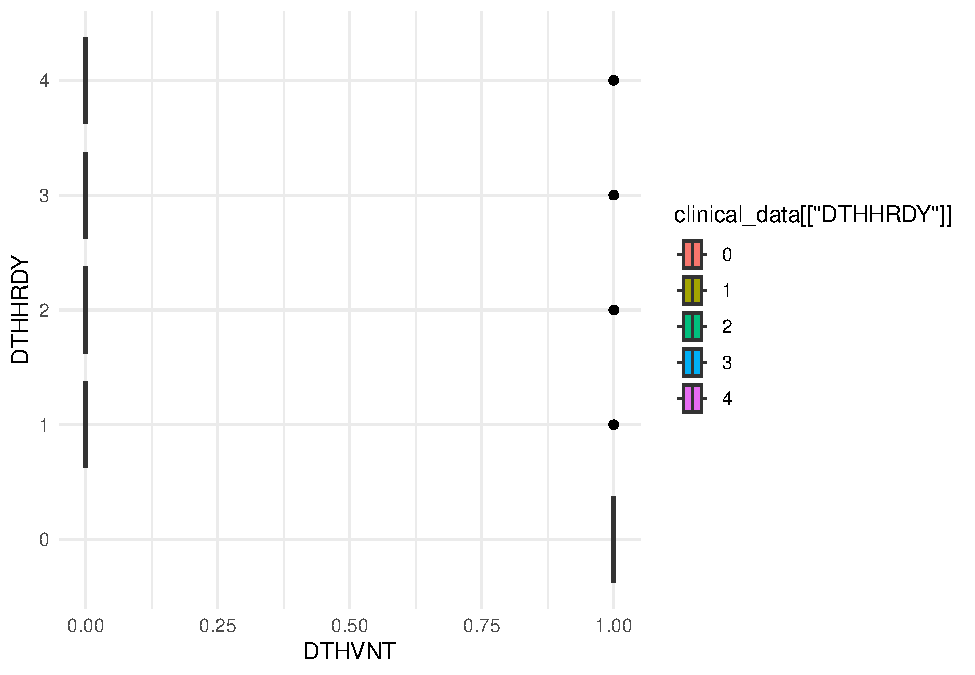
\includegraphics{Q1_markdown_files/figure-latex/unnamed-chunk-8-13.pdf}

\hypertarget{principal-components-analysis-pca}{%
\subsubsection{Principal Components Analysis
(PCA)}\label{principal-components-analysis-pca}}

\begin{verbatim}
## Warning in PCA(pca_df, graph = TRUE): Missing values are imputed by the mean of
## the variable: you should use the imputePCA function of the missMDA package
\end{verbatim}

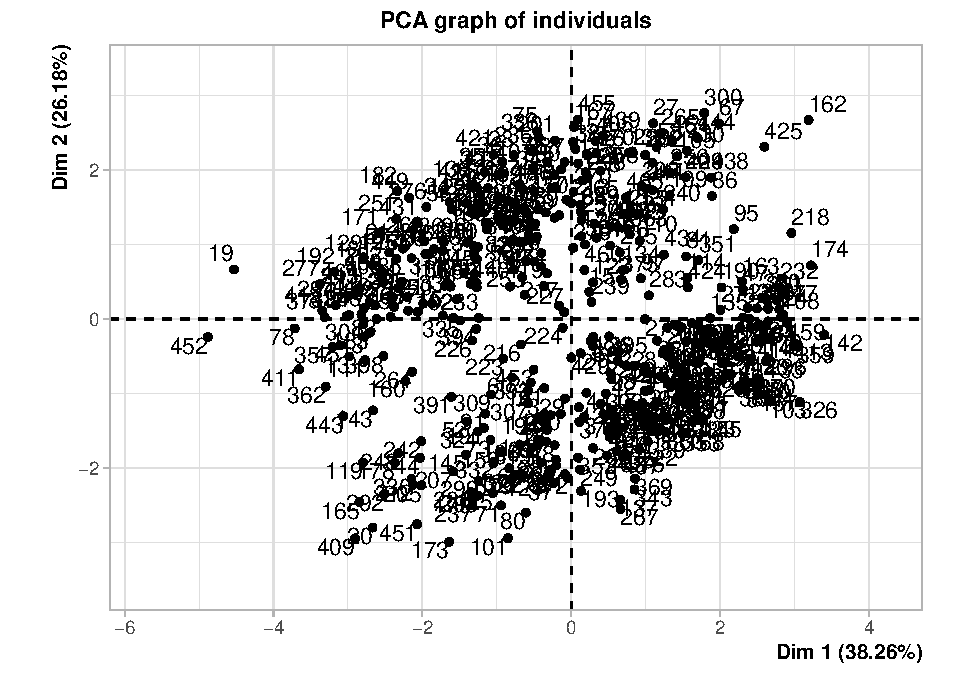
\includegraphics{Q1_markdown_files/figure-latex/unnamed-chunk-9-1.pdf}
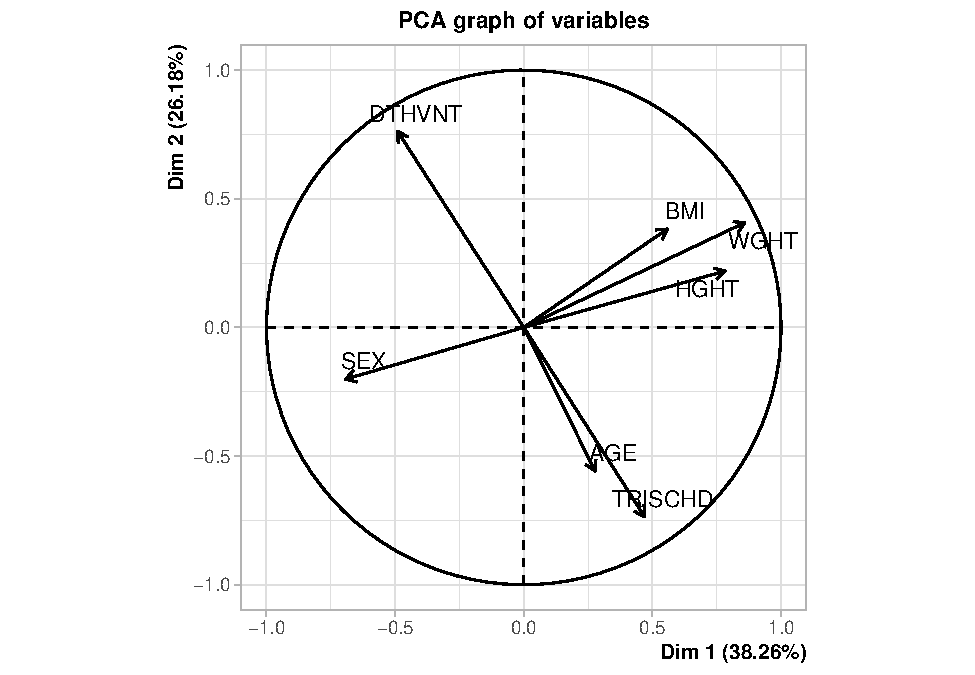
\includegraphics{Q1_markdown_files/figure-latex/unnamed-chunk-9-2.pdf}
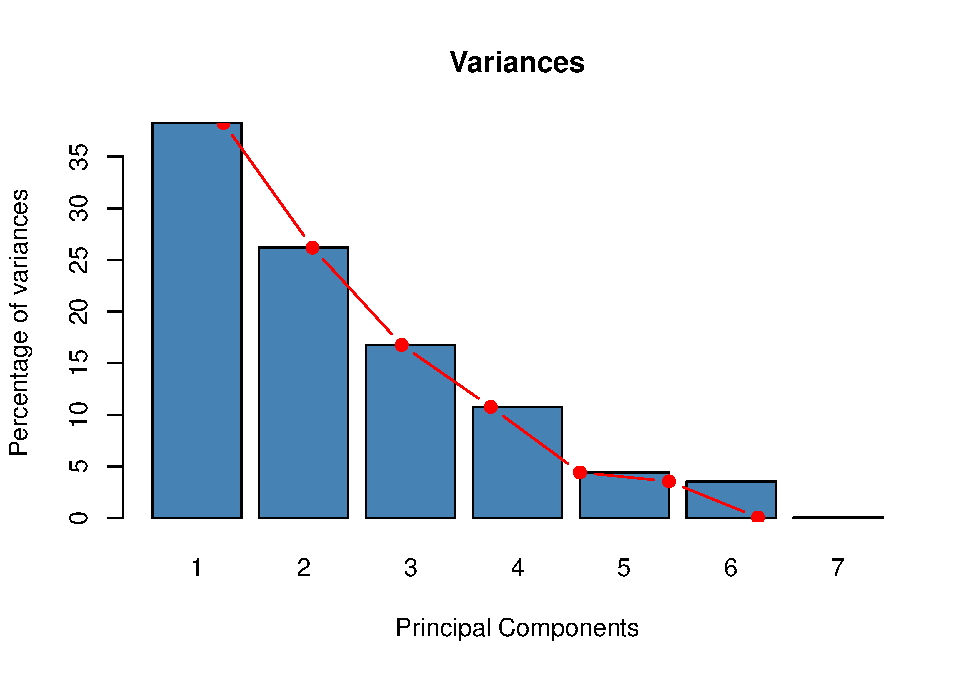
\includegraphics{Q1_markdown_files/figure-latex/unnamed-chunk-9-3.pdf}
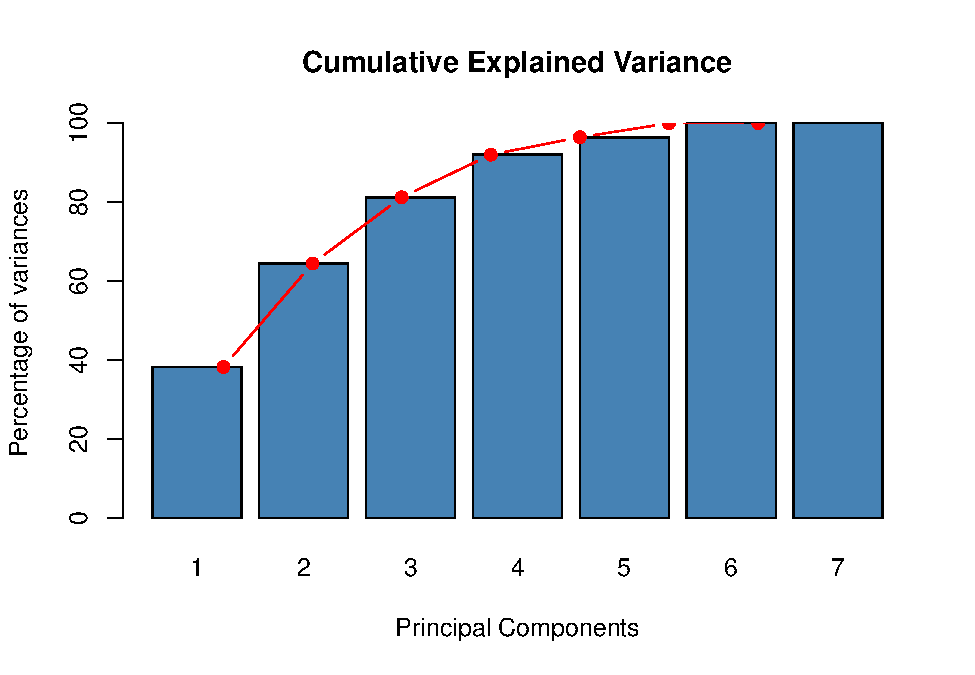
\includegraphics{Q1_markdown_files/figure-latex/unnamed-chunk-9-4.pdf}

\hypertarget{multiple-factor-analysis-mfa}{%
\subsubsection{Multiple Factor Analysis
(MFA)}\label{multiple-factor-analysis-mfa}}

\begin{verbatim}
## Warning: ggrepel: 6 unlabeled data points (too many overlaps). Consider
## increasing max.overlaps
\end{verbatim}

\includegraphics{Q1_markdown_files/figure-latex/unnamed-chunk-10-1.pdf}
\includegraphics{Q1_markdown_files/figure-latex/unnamed-chunk-10-2.pdf}

\begin{verbatim}
## Warning: ggrepel: 463 unlabeled data points (too many overlaps). Consider
## increasing max.overlaps
\end{verbatim}

\includegraphics{Q1_markdown_files/figure-latex/unnamed-chunk-10-3.pdf}
\includegraphics{Q1_markdown_files/figure-latex/unnamed-chunk-10-4.pdf}

\begin{verbatim}
## Warning: ggrepel: 441 unlabeled data points (too many overlaps). Consider
## increasing max.overlaps
\end{verbatim}

\includegraphics{Q1_markdown_files/figure-latex/unnamed-chunk-10-5.pdf}
\includegraphics{Q1_markdown_files/figure-latex/unnamed-chunk-10-6.pdf}
\includegraphics{Q1_markdown_files/figure-latex/unnamed-chunk-10-7.pdf}
\includegraphics{Q1_markdown_files/figure-latex/unnamed-chunk-10-8.pdf}
\includegraphics{Q1_markdown_files/figure-latex/unnamed-chunk-10-9.pdf}

\end{document}
